

\subsection{Overview}
The instruction planner is placed at the top layer of the whole SmartSoft architecture,
therefore it is meant to be the "Swarm Manager" of all Robots that work on a common Task. \\
This approach has been split up into two different aspects, one part of the Instruction planner has to
observe all robots and the states that they are currently in, as well as the task that they are working on.
While the other part of the Instruction planner needs to keep up with the progress on the objective, to
predict and estimate the proximate steps to the goal.

\subsection{Idea}

The following Picture \ref{fig:instr_overview} shows the internal structure of the
instruction planner.
As seen in the Picture the instruction planner will do multiple things: \newpage
In Blue:\\
\begin{itemize}
    \item \textbf{Game Management:}  organization of next steps
    \begin{itemize}
        \item Exploration Management
            \begin{itemize}
                \item keeps log of found machines
                \item estimates explorable positions
                \item suggests next orders to reach the objective
            \end{itemize}
        \item Production Management
        \begin{itemize}
            \item coming up
        \end{itemize}
    \end{itemize}
    \item \textbf{Fleet Management:} organization of robots and their progress
    \begin{itemize}
        \item which state they are in (e.g disqualified / maintenance / active)
        \item what they are working on
        \item error handling
    \end{itemize}
\end{itemize}

\begin{figure}[h]
\centering
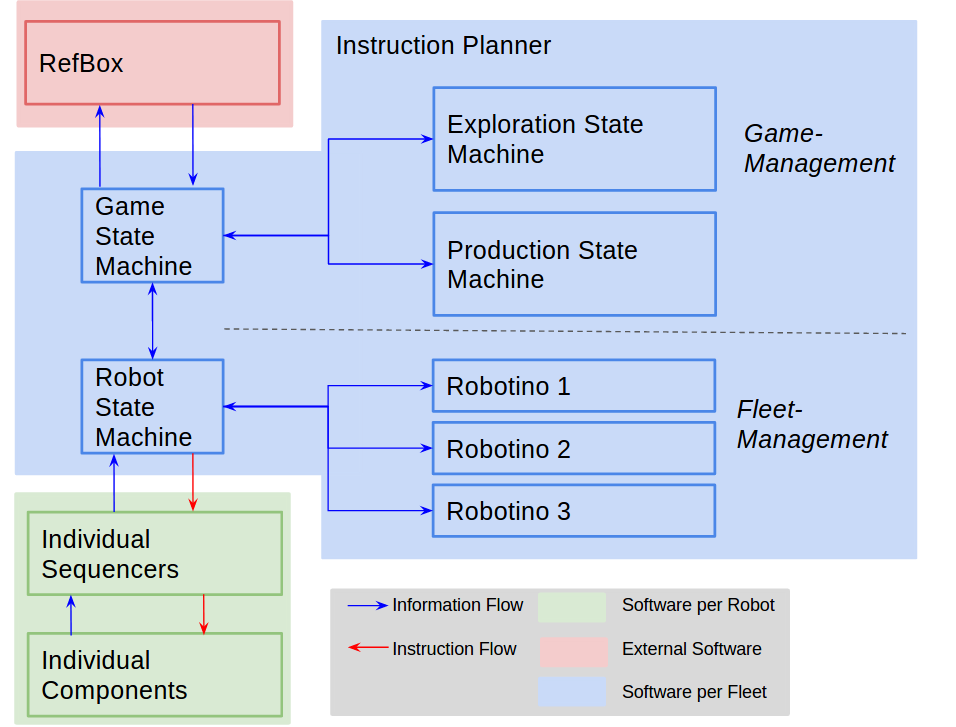
\includegraphics[scale=0.23]{pic/Instructionplanner2018.png}
\caption{Management of Robot Swarm and the Objective}
\label{fig:instr_overview}
\end{figure}
\newpage

Since the Blue-part of figure \ref{fig:instr_overview} handles the internal management
it can be treated at as an agent that provides the next orders for the robots, based
on their actual situation.\\
This situation is brought into the instruction planner via the Sequencers of each
robot.
In Green: \\
\begin{itemize}
    \item \textbf{Sequencers}
    \begin{itemize}
        \item handle all events on robot
        \item local management of robot
    \end{itemize}
    \item \textbf{Components}
    \begin{itemize}
        \item actual hardware
        \item creates events
    \end{itemize}
\end{itemize}


\subsubsection{Objective Management}
The objective management consists of multiple \textit{state machine}, that are in
a hierarchical order.
All state machines listen to the events that are received via the \textit{sequencers}, or
the \textit{refbox}.
The thought behind this architecture is an intelligent agent that can be "asked" for the next
best step to take.\\

The game state machine is a first level state machine that takes care of the current
game phase, (e.g. exploration phase, production phase, pause, etc. ). depending on the phase the
events are then forwarded to the next level state machines, such as the exploration state machine. \\
\\
The exploration state machine takes then care of all objectives that have to be fulfilled in the
exploration phase.
\subsubsection{Fleet Management}


The

\subsection{Changes}
Previously the purpose of the instruction planner was misunderstood, so the whole structure of
this component had to be planned again. \\
The implementation now differs a lot from the old of 2017. Only view lines of code could be recycled and used again.
A completely new system has been introduced: the \textit{hierarchical state machines}. The implementation of
this system now is more modular, parts (e.g. the state machines for the phases) can easily be exchanged and
replaced with other approaches or implementations. \\
Also new is the split of tasks into \textit{Fleet Management} and \textit{Objective Management}. This
allows the system to be even more flexible, since commendation of the robot is now isolated from the Task that the
Swarm should perform. \\
\\
Overall the instruction planner has been completely redesigned and is still under construction.
The basic ideas are implemented but still need to be filled with "live".

\subsection{Conclusion}
With the new architecture of the instruction planner multiple new features can be implemented.
\begin{itemize}
    \item \textbf{Multiple Robots} The new implementation would allow the use of multiple robots on the field, since
    the new architecture considers the use of multiple sequencers.
    \item \textbf{Intelligent Agents} The \textit{Objective Management} is designed to work with agents that can be asked
    for the next steps, in the actual case the implementation works with state machines. Other implementations of Agents can
    also be fit into the interface.
    \item \textbf{divide et impera} Separating the robot management form the objective management separates two problems
    that can be handled individually: \textit{Objective Manager} creates the next task and the \textit{Fleet Manager} takes care
    of all robots and assigns this task to the best candidate.
\end{itemize}

The actual level of Production does not contain a fully functional instruction planner.
The current state consists of the skeleton of the parts, the implementation of the
actual agent is missing as well as the logic to distribute the tasks to multiple Robots.
The Architectural changes allow to start the work on any part of the system since the would not affect each other,
while still just some implementation is necessary for the whole code to work.
Probably the first implementations of the \textit{Objective Manager} might be a
simple static implementation of a point pattern to follow, as well as a simple \textit{Fleet Manager} that
assigns just one order at a time to only onre Robot.


\subsection{Testing}
The instruction planner is still under construction and therefore untested.
Especially the use of Multiple Robotinos could not be tested and is not planned to take action in the upcoming contest.

\newpage
